%%%%%%%%%%%%%%%%%%%%%%%%%%%%%%%%%%%%%%%%%
% University/School Laboratory Report
% LaTeX Template
% Version 3.1 (25/3/14)
%
% This template has been downloaded from:
% http://www.LaTeXTemplates.com
%
% Original author:
% Linux and Unix Users Group at Virginia Tech Wiki 
% (https://vtluug.org/wiki/Example_LaTeX_chem_lab_report)
%
% License:
% CC BY-NC-SA 3.0 (http://creativecommons.org/licenses/by-nc-sa/3.0/)
%
%%%%%%%%%%%%%%%%%%%%%%%%%%%%%%%%%%%%%%%%%

%----------------------------------------------------------------------------------------
%	PACKAGES AND DOCUMENT CONFIGURATIONS
%----------------------------------------------------------------------------------------

\documentclass{article}

\usepackage[version=3]{mhchem} % Package for chemical equation typesetting
\usepackage{siunitx} % Provides the \SI{}{} and \si{} command for typesetting SI units
\usepackage{graphicx} % Required for the inclusion of images
\usepackage{natbib} % Required to change bibliography style to APA
\usepackage{amsmath} % Required for some math elements 
\usepackage{enumerate} % Required for the enumerate function
\usepackage[siunitx]{circuitikz} % Required for the drawing of circuit diagrams
\usepackage{caption}
\usepackage{graphicx}
\usepackage{subcaption}
\usepackage{xfrac}
\usepackage{float}
\usepackage{enumitem}
\usepackage{chemgreek}
\usepackage{booktabs}
\usepackage{epstopdf}
\usepackage{pgfplots}

\setlength\parindent{0pt} % Removes all indentation from paragraphs

\renewcommand{\labelenumi}{\alph{enumi}.} % Make numbering in the enumerate environment by letter rather than number (e.g. section 6)

%\usepackage{times} % Uncomment to use the Times New Roman font

\graphicspath{{./fig/}}

%----------------------------------------------------------------------------------------
%	DOCUMENT INFORMATION
%----------------------------------------------------------------------------------------

\title{Electrical Machines \& Power Systems \\ Practical 3 - Synchronous Machines \\ ENG224} % Title

\author{Shane \textsc{Reynolds}} % Author name

\date{October 1, 2016} % Date for the report

\begin{document}

\maketitle % Insert the title, author and date

\begin{center}
\begin{tabular}{l r}
Date Performed: & September 10, 2016 \\ % Date the experiment was performed
Instructor: & Dr Kamal Debnath % Instructor/supervisor
\end{tabular}
\end{center}

% If you wish to include an abstract, uncomment the lines below
% \begin{abstract}
% Abstract text
% \end{abstract}

%----------------------------------------------------------------------------------------
%	SECTION 1
%----------------------------------------------------------------------------------------

\section{Objective}

Using a dc motor as a prime mover, synchronous machine will be operated as an alternator. Equivalent circuit parameters will be obtained using open circuit and short circuit tests. Phasor diagrams will be drawn for each testing scenario to aid analysis. 
 
%----------------------------------------------------------------------------------------
%	SECTION 2
%----------------------------------------------------------------------------------------

\section{Procedure and Results}
\subsection{Open circuit test}

The open circuit test is carried out with the terminals of the synchronous machine disconnected, as shown in the equivalent circuit model of the synchronous machine in Figure 1. In this test, there is no armature current the measured terminal voltage, $V_t$, is the induced voltage, $E_f$.

 \begin{figure}[h]
 	\centering
 	\ctikzset{bipoles/length=0.8cm}
 	\begin{circuitikz}[american voltages]
 		\draw (0,0)
 		to [sV,l=$E_f$] (0,2)
 		to [L,l=$X_s$,i=$I_a$] (2,2)
 		to [R,l=$R_a$,-o] (4,2)
 		;
 		\draw (0,0)
 		to [short,-o] (4,0)
 		;
 		\draw (4,1)
 		to [short,l_=$V_t$] (4,1)
 		;
 	\end{circuitikz}
 	\caption{Synchronous generator equivalent circuit}
 \end{figure}
 
 The synchronous machine was connected in a star, and the DC motor was engaged to run the synchronous machine at rated speed of 1500 rpm. Readings of the field current and the open circuit line to neutral voltage were recorded. The experimental results can be seen in Table 1.
 
 \begin{minipage}{\textwidth}
 	\begin{minipage}[b]{0.49\textwidth}
 		\centering
 		\begin{tabular}{rr}
 			\toprule
 			$I_f$ ($\si{\ampere}$) & $E_f$ ($\si{\volt}$)\\
 			\midrule
 			0.000 & 5.50 \\
 			0.210 & 23.50 \\
 			0.037 & 40.00 \\
 			0.073 & 81.00 \\
 			0.110 & 120.50 \\
 			0.157 & 160.00 \\
 			0.212 & 200.00 \\
 			0.246 & 220.00 \\
 			0.324 & 254.00 \\
 			\bottomrule
 		\end{tabular}
 		\captionof{table}{Experimental results\\ of open circuit test}
 	\end{minipage}
 	\hfill
 	\begin{minipage}[b]{0.49\textwidth}
 		\centering
 		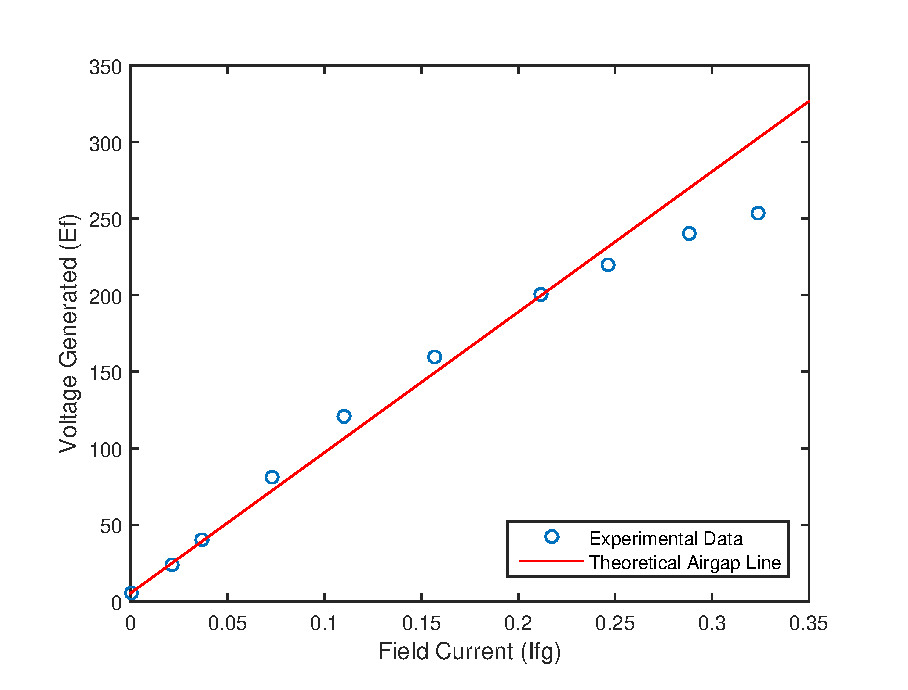
\includegraphics[scale=0.45]{fig1}
 		\captionof{figure}{Open circuit \\characteristic plot}
 	\end{minipage}
 \end{minipage}
 
 \vspace{1cm}
 
 The open circuit characteristic plot can be seen in Figure 2. We note that the field current for which the rated voltage (240V) is generated is:
 \begin{center}
 	\fbox{$I_{f0} = 0.288\si{\ampere}$}
 \end{center}
 
 To find an equation of the theoretical air gap line, shown in Figure 2, two $I_f$ and $E_f$ tuples were used to find the equation:
 \begin{align}
	 E_f = 917.45 \cdot I_f + 5.5
 \end{align}  
 
\subsection{Short circuit test}

The short circuit test is carried out with the terminals of the machine short circuited. Figure 3 shows the equivalent circuit for the test. The field current was set to zero, and the synchronous generator was driven by the DC machine at synchronous speed. The field winding current was slowly increased until the short circuit armature current reached the rated current.

\begin{figure}[h]
	\centering
	\ctikzset{bipoles/length=0.8cm}
	\begin{circuitikz}[american voltages]
		\draw (0,0)
		to [sV,l=$E_f$] (0,2)
		to [L,l=$X_s$,i=$I_a$] (2,2)
		to [R,l=$R_a$,-o] (4,2)
		;
		\draw (0,0)
		to [short,-o] (4,0)
		;
		\draw (4,2)
		to [short,o-o] (4,0)
		;
	\end{circuitikz}
	\caption{Synchronous generator equivalent circuit}
\end{figure}
\newpage
The short circuit current, $I_{sc0}$, at the rated voltage of 240$\si{\volt}$ was found to be:
\begin{center}
	\fbox{$I_{sc0} = 0.318\si{\ampere}$}
\end{center}
\vspace{0.5cm}
This point was plotted on the against the rated armature current, $I_a$, and can be seen in Figure 3 with the short circuit characteristic curve (SCC).

\begin{figure}[H]
	\centering
	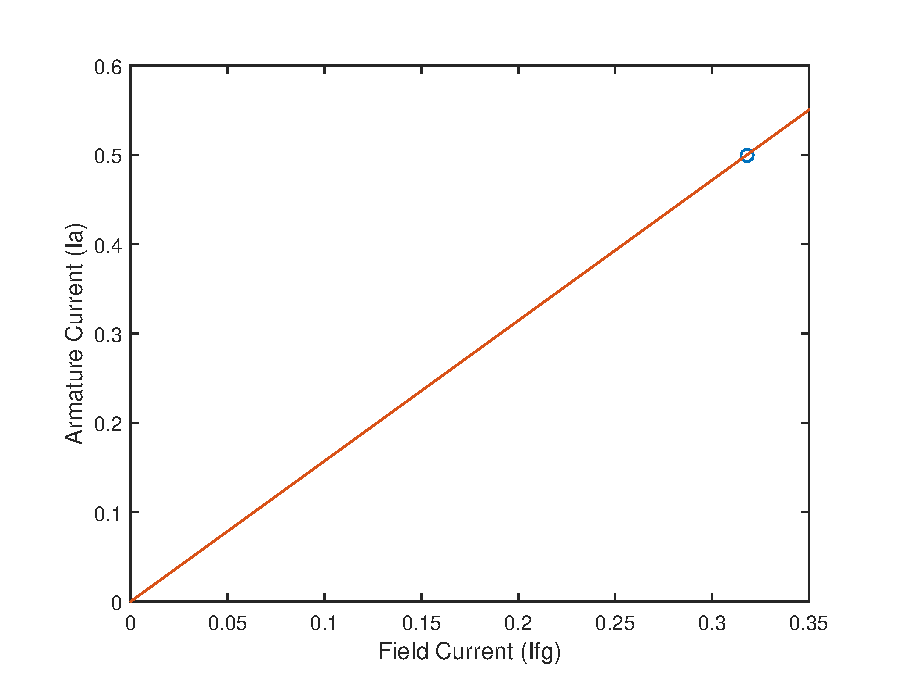
\includegraphics[scale=0.5]{fig2}
	\caption{The short circuit characteristic plot.}
\end{figure}

The equation of the SCC, was found using simple coordinate geometry and is reported as:
\begin{align}
	I_a = 1.572 \cdot I_f
\end{align}

The field current at the rated voltage, $I_f$, found in the open circuit test is used in conjunction with equation (1) and equation (2) to find the synchronous impedence, $Z_s$.
\begin{align*}
	Z_s = \frac{917.45 \cdot 0.288 + 5.5}{1.572 \cdot 0.288} = 595.76\si{\ohm}
\end{align*}

The saturated synchronous impedence, is:
\begin{center}
	\fbox{$Z_s = 595.76\si{\ohm}$}
\end{center}

\subsection{Stator resistance}
The stator resistance was found by passing a current of $0.5\si{\ampere}$ through the stator windings and recording a voltage of $23.75\si{\volt}$. The stator winding resistance was measured as:
\begin{center}
	\fbox{$R_a = 49\si{\ohm}$}
\end{center}
\vspace{0.5cm}
We can find the saturated synchronous reactance, $X_s$, since $Z_s = R_a +jX_s$:
\begin{align*}
	X_s = \sqrt{Z_s^2 - R_a^2} = 593.74\si{\ohm}
\end{align*}

Hence, the saturated synchronous reactance is given by:
\begin{center}
	\fbox{$X_s = 593.74\si{\ohm}$}
\end{center}

\subsection{Phasor diagrams}

Phasor diagrams for both the open circuit test and the short circuit test can be seen in Figures 5 and 6.

\begin{figure}[h]
	\begin{minipage}{.5\textwidth}
		\begin{tikzpicture}
		\begin{axis}[
		xmin=0,
		xmax=350,
		ymin=-125,
		ymax=125,
		axis lines = none,
		xlabel = $Re$,
		ylabel = {$Im$}
		]
		
		\addplot [blue, no markers, ->] coordinates {(0,0) (240,0)} node[below,pos=1] {$V_t = E_f$};
		
		
		\end{axis}
		\end{tikzpicture}
		\caption{Phasor diagram for\\ open circuit test}
	\end{minipage}
	\begin{minipage}{0.5\textwidth}
		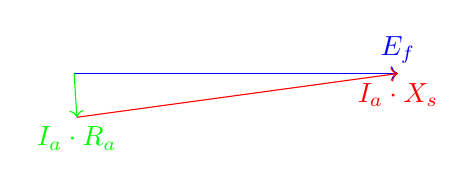
\begin{tikzpicture}
		\begin{axis}[
		xmin=-50,
		xmax=350,
		ymin=-125,
		ymax=125,
		axis lines = none,
		xlabel = $Re$,
		ylabel = {$Im$}
		]
		
		\addplot [blue, no markers, ->] coordinates {(0,0) (240,0)} node[above,pos=1] {$E_f$};
		\addplot [green, no markers, ->] coordinates {(0,0) (2.01,-24.41)} node[below,pos=1] {$I_a \cdot R_a$};
		\addplot [red, no markers, ->] coordinates {(2.01,-24.41) (240,0)} node[below,pos=1] {$I_a \cdot X_s$};
		
		
		\end{axis}
		\end{tikzpicture}
		\caption{Phasor diagram for\\ short circuit test}
	\end{minipage}
\end{figure}

We see that in Figure 5 $V_t$ is the same as $E_f$ due to the fact that there is no current $I_a$ since the circuit is open. Similarly, we note that since there is no load attached to the generator, the is no terminal voltage (because it's shorted).
%----------------------------------------------------------------------------------------
%	SECTION 4
%----------------------------------------------------------------------------------------

\section{Conclusion}
Using a dc motor as a prime mover, synchronous machine was operated as an alternator. The following equivalent circuit parameters were obtained using open circuit and short circuit tests:

\begin{align*}
	R_a &= 49\si{\ohm}\\
	Z_s &= 593.74\si{\ohm}
\end{align*}
\end{document}